
\chapter{Dataset preparation}

\begin{introduction}
In this chapter, it will be discussed various ways of applying artificial intelligence models to archaeology.
\end{introduction}





Deep learning is a subtype of artificial intelligence, which relies on neural networks in order to recognize patterns in given training data. When trained on a dataset, the network is able to learn many features of the dataset, becoming able to make predictions when presented with new data.


%One of the pillars of deep learning is the diversity of the dataset, and also the precision of the training annotations, because the model will be able to learn small possible variations in the data, reducing the risk of overfitting, therefore a good dataset is fundamental, however it is not always possible to obtain a dataset that represents all the input possibilities.

%\subsubsection{Overfitting}
%Overffiting occurs when a model performs very well on training data, yet when presented with new data has difficulty making correct predictions. This can occur for several reasons:
%\begin{itemize}
%\item There is too little training data, creating a dataset that is unrepresentative of all possible inputs.
%
%\item The model is trained for a long time and thus, without stopping early, increasingly makes the model only an expert on the given type of training data.
%
%\item The model is too complex, causing it to learn not only the necessary predictive features, but also the noise that the inputs may have.
%\end{itemize}

To perform the Odyssey project, the Alto Minho region, Portugal, was chosen. With the help of the Comunidade Intermunicipal do Alto Minho, LiDAR data of 2018 was collected, covering 2220 km2, being later applied the visualization technique, more specifically LRM. As a result of this process 4 LRM images were generated, corresponding to 4 sub-regions of Alto Minho: Viana do Castelo, Paredes de Coura, Arcos de Valdevez and Parque Nacional da Peneda-Gêrez, with each pixel corresponding to 0.5 meters on the terrain.
From these 4 sub-regions, the locations of all known tumuli and castros were also noted.

The following table shows the resolution of each image, as well as the number of known annotations and the image size.

\begin{table}[h!]
\centering
\begin{tabular}{|p{3cm}|p{2.5cm}|p{2cm}|p{2cm}|p{2cm}|} 
 \hline
  Region & Resolution(px) & Annotations (tumulis) & Annotations (hillforts) & Size (GB) \\ [0.5ex] 
 \hline\hline
 Viana do Castelo & 19,978x46.000 & 14 & 41 & 3.7\\ 
 Paredes de Coura & 13,999x51,999 & 56 & 65 & 2.9 \\
 Arcos de Valdevez & 15,999x43,999 & 71 & 46 & 2.8\\
 Parque Nacional da Peneda-Gerês & 19,999x44,955 & 135 & 11 & 3.6\\ [1ex] 
 \hline
\end{tabular}
\caption{Description of the dataset used}
\end{table}

The following image shows the joint of the 4 LRM images, corresponding to the entire Alto Minho area where LiDAR data was collected.

\begin{figure}[H]
\centering
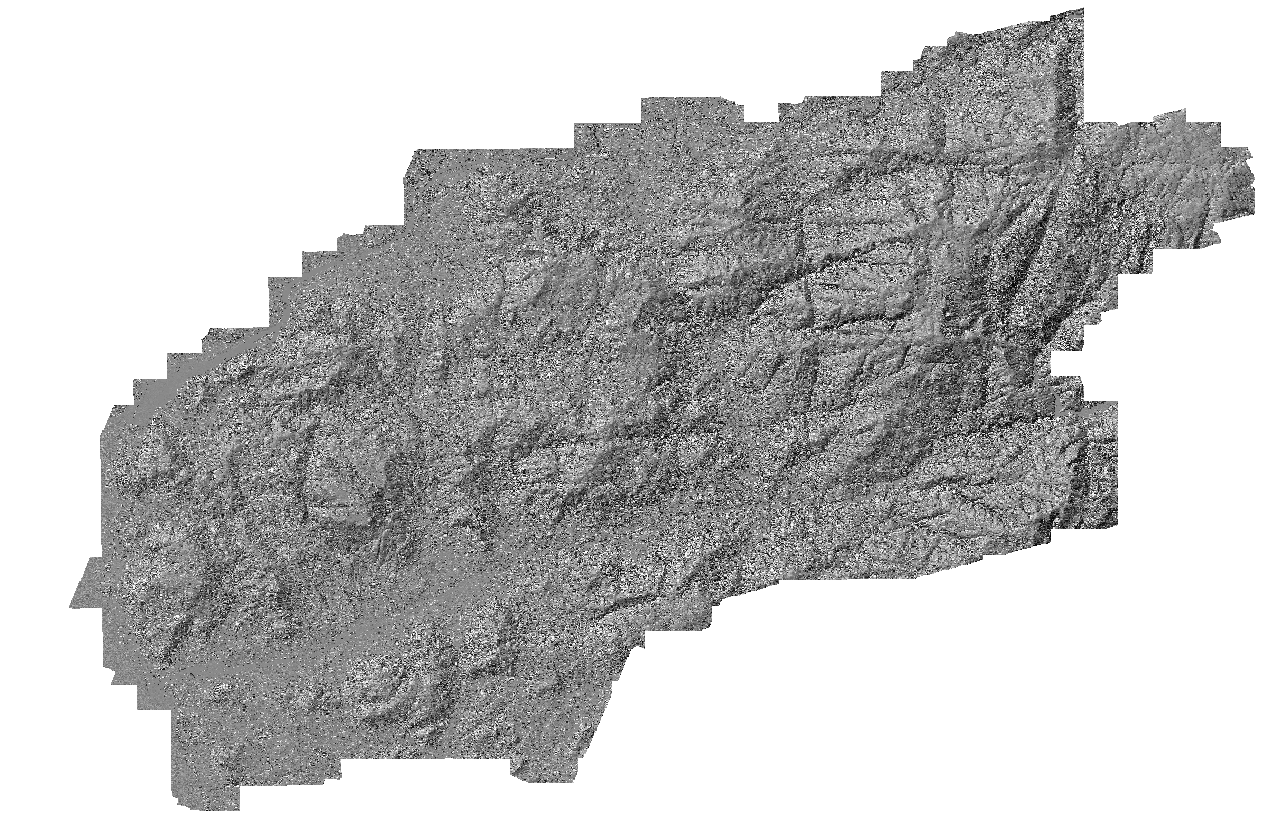
\includegraphics[width=10cm]{images/LRMfinal.png}
\caption{The 4 LRM images together, corresponding to Alto Minho}
\end{figure}





%That said, in this project the amount of data provided is relatively small \cite{yolov5recomedacoes}, as you can see, it is recommended to use for each type of object more than 1500 images and more than 10000 annotations to have good results, and since YOLOv7 is a relatively large model, this is even more important, due to the possibility of the weights not converge all if the dataset is small, and that is what this section is about, creation of the dataset, as well its augmentation.

\subsection{Creation of the base dataset}

With the LRM images, the locations of known tumuli and hillforts were provided in the Well-Know Text (WKT) format. This format indicates in polynomial form the geographical location of the site in question.

However, as it is possible to see from the table above, the 4 LRM images are too large, both for training the YOLOv7 model and the Unet model. Because of this, the 4 images were processed in order to obtain a dataset with 640x640 pixels images, being a typical size to train both YOLOv7 and Unet.

For this, a Python script was used. In this script, one LRM image was loaded at a time, as well as its annotations. To simplify it, separate datasets were generated for the tumuli and for the forts. Then, the annotations were parsed, and using the LRM image metadata, the geographic coordinates of the image extremities were obtained. With that, the coordinates present in the annotation polynomials were converted to pixels using the mapping function, as illustrated below:

\begin{equation}
     pixel = \frac{(coordenate - inMin) * (outMax - outMin)} {(inMax - inMin)} + outMin
     \label{Map function}
\end{equation}

In the function, the inMin and inMax represent the geographic coordinates of the LRM image extremities, whereas the outMin and outMax represent the size of the image in pixels. However, in the y-coordinate, are counted from top to bottom. Therefore, to calculate the y-coordinate of the pixel, outMin and outMax are swapped.


As previously stated, 4 LRM images have been provided as well as the annotations of where the archaeological sites are located. In order to generate the dataset, a python script was used. From the 276 tumuli provided, 161 images were generated, each image containing between 1 and 9 tumuli, for the hillforts 150 images were created, containing 152 sites, each image containing between 1 and 2 hillforts. With the same script, .las files were also generated, for each annotation, each file only contains the points of the cloud of points corresponding to the object in question, this files will be later use to train a machine model, with the objective to validate the results from the YOLOv7. Note that the annotations in the YOLOv7 format, follow the following format, annotation type, center point (x, y), width and height, both the center point and the measures are normalized.

Initially the annotations were transformed from GIS reference to pixels and then into boundind boxes, because the provided annotations came segmented, i.e. in the form of polygons as shown in the figure below.

\begin{figure}[H]
\centering
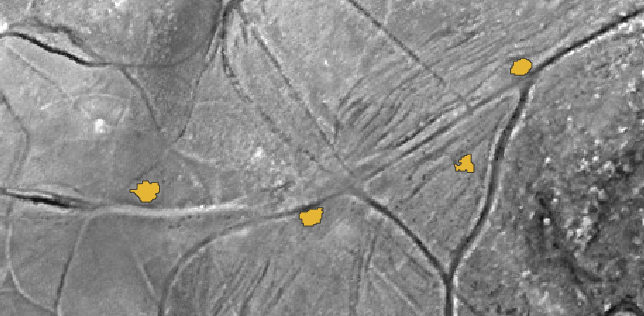
\includegraphics[width=10cm]{images/segmentacao_mamoas.png}
\caption{Original annotations}
\end{figure}
It is worth to mention that each pixel corresponds to 0.5 meters in the ground.

After that, for each bounding box not yet processed, the script randomizes a position for the object inside a 640x640 pixel image, if all objects are completely inside the image, the image is generated as well as its labels.

As can be seen, the number of annotations are far from the ideal, so two algorithms were used to generate an augmented datasets.

\subsection{Augmentation copy paste}

The first augmentation algorithm, which I will refer to as copy-paste augmentation.

The copy paste algorithm consists in copying objects (tumuli or hillforts) to other areas, creating a larger dataset.

For this algorithm, a deep learning model, YOLOv5, was trained with only the initial data, and a topographic chart of the area under study was also used. 

Initially it was performed the cropping of the annotations with the segmentation, having the objects cropped was applied one of the following geometric transformations, flip left to right, flip top to bottom, rotate 90, 180 or 270 degrees and transpose.
Once this is done, random areas were selected where there are no annotations, which were then passed on the trained model only with the original dataset, to make sure that there are no undetected objects in that area. 

After this the object is pasted and to be sure that the image is not pasted on top of buildings, houses, rivers, roads, etc (areas where there would never be an object to detect), a topographic map of the area under study (Viana do Castelo) is used in order to check if the randomly selected zone can be chosen. At the end the final 640x640 pixels images are generated together with the text files containing the labels.

\begin{figure}[H]
\centering
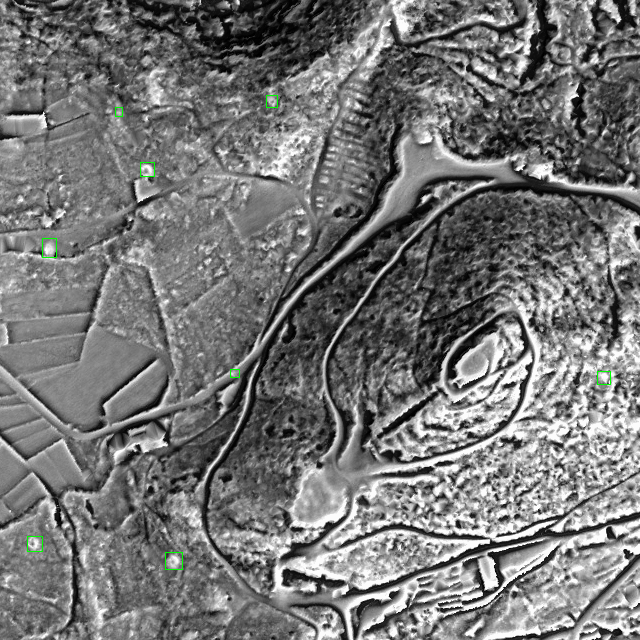
\includegraphics[height=9cm]{images/mamoas_aug_example.png}
\caption{Example of copy paste augmentation}
\end{figure}

\subsection{Simple augmentation}
The second augmentation algorithm, which will be called simple augmentation, which as the name indicates, is much simpler than the first one, this one is based on centering each object in a 640x640 pixels box and moving the box randomly, after that verify if the object is completely inside the box, as well as other nearby objects, if all the objects are inside the box, one of the same transformations of the previous algorithm is applied, but not to the object itself but to the image, finally the images are saved as well as the labels

This way it is possible to have the same annotation but in a different position of the image, with different backgrounds.

\subsection{Augmentation results}

Analyzing the github repository which contains the code needed to run YOLOv7, is possible to verify that no recommendations for creating a custom dataset are indicated, not even in the published paper \cite{paperyolov7}, in which it is only indicated that the COCO dataset was used to train the model and nothing else is mentioned about datasets. 

However in the YOLOv5 repository, there is a section, where it is given recommendations on how to train a custom dataset, and as said before, it is recommended per object type to have more than 1500 images and more than 10000 annotations \cite{yolov5recomedacoes}.

Following this recommendation for the copy paste increase, a dataset was generated for the 2754 images containing a total of 18398 tummies, noteworthy that within these 2754, 130 are from the original dataset.

For the simple augmentation, not as many as recommended were used, 1380 images were generated, with a total of 3124 tummies.

For the hillforts, with copy paste augmentation, 2464 images were generated, with a total of 6925, also here the 140 images are from the original dataset. Here the number of castros was reduced a little, not reaching the recommended 10000, due to their size, usually large objects, the image would be too populated and unrealistic.

For the simple augmentation 815 images were generated with a total of 844 hillforts.

FALTA AQUI alterar o numero dos castros que estao mal
